\documentclass[10pt, a4paper]{article}
\usepackage[left=3.17cm, right=3.17cm, top=2.54cm, bottom=2.54cm]{geometry}
\usepackage[UTF8]{ctex}
\usepackage{amsmath}
\usepackage{amsfonts}
\usepackage{amssymb}
\usepackage{mathrsfs}
\usepackage{enumerate}
\usepackage{caption}
\usepackage{graphicx}
\usepackage{subfig}
\usepackage{siunitx}
\usepackage{minted}
\usemintedstyle{rainbow_dash}
% \usepackage{fontspec}
\setmonofont[]{Fira Code}
\usepackage{hyperref}
\hypersetup{unicode, colorlinks=true, linkcolor=black, urlcolor=blue}

\begin{document}
\definecolor{bg}{rgb}{0.95,0.95,0.95}

\title{Matlab\,图像处理实验报告}
\author{暮月}

\maketitle

\tableofcontents

\paragraph{环境与依赖说明}本次实验使用的是Matlab R2020a Update3,主要使用了Image Processing Toolbox 11.1、Computer Vision Toolbox 9.2和Parallel Computing Toolbox 7.2。Matlab设置为使用utf-8编码,所有代码文件无特殊情况均为此编码,注释以英文为主。

\section{基础知识}
\subsection{练习题}
\textbf{利用MATLAB提供的函数完成以下任务}
\begin{enumerate}[(a)]
    \item 以测试图像的中心为圆心,图像的长宽中较小值的一半为半径画一个红颜色的圆

          经在文档中搜索,Computer Vision Toolbox中存在函数\mintinline{matlab}{insertShape}可以直接在图像中绘制圆形。下方代码用于绘制满足要求的一个红色半透明圆形:

          \begin{minted}[bgcolor=bg]{matlab}
[h, w, c] = size(img);

pos = [[w, h] / 2, min([w, h] / 2)];
img_circle = insertShape(img, 'Circle', pos, ...
                         'color', 'red', 'Opacity', 1);
          \end{minted}

          此外,还可以通过圆的一般方程或者参数方程绘制:

          \begin{minted}[bgcolor=bg]{matlab}
circle_mask = ((x-pos(1)).^2 + (y-pos(2)).^2 >= pos(3).^2+60) ...
               |((x-pos(1)).^2 + (y-pos(2)).^2 <= pos(3).^2-60);
img_circle = img .* circle_mask;
img_circle(:,:,1) = img_circle(:,:,1) + ~circle_mask;

phi = 0:1:359;
x_ = max(min(round(pos(1) + pos(3) * cos(phi)), w), 1);
y_ = max(min(round(pos(2) + pos(3) * sin(phi)), h), 1);
img_circle = img;
img_circle(sub2ind(size(img), y_, x_, ones(1, 360))) = 1;
img_circle(sub2ind(size(img), y_, x_, 2 * ones(1, 360))) = 0;
img_circle(sub2ind(size(img), y_, x_, 3 * ones(1, 360))) = 0;
          \end{minted}

    \item 将测试图像涂成国际象棋状的“黑白格”的样子,其中“黑”即黑色,“白”即意味着保留原图

          只需构造一个分块为1或0的矩阵,再与图像矩阵进行逐元素乘,便可让图像分块。即类似:
          \begin{align*}
              \text{Img} .*
              \begin{bmatrix}
                  1      & \cdots & 1      & 0      & \cdots & 0      \\
                  \vdots & \ddots & \vdots & \vdots & \ddots & \vdots \\
                  1      & \cdots & 1      & 0      & \cdots & 0      \\
                  0      & \cdots & 0      & 1      & \cdots & 1      \\
                  \vdots & \ddots & \vdots & \vdots & \ddots & \vdots \\
                  0      & \cdots & 0      & 1      & \cdots & 1      \\
              \end{bmatrix}
              =
              \begin{bmatrix}
                  \text{Img}_1 & 0            \\
                  0            & \text{Img}_2
              \end{bmatrix}
          \end{align*}

          故只需将每个像素的坐标先除以格宽,再对2求余,便可以得到横纵方向上的01分布。然后将这个01分布进行异或,便可以得到一个01组成的块相间分布的矩阵。最后与图像矩阵进行逐元素乘得到所需结果。核心代码如下:

          \begin{minted}[bgcolor=bg]{matlab}
[x, y] = meshgrid(1:w, 1:h);

grid_width = 10;
x_mask = mod(floor(x / grid_width), 2);
y_mask = mod(floor(y / grid_width), 2);
grid_mask = double(xor(x_mask, y_mask));
img_grid = grid_mask .* img;
          \end{minted}
\end{enumerate}

最终结果如图\ref{fig:exp1}

\begin{figure}[ht!]
    \centering
    \subfloat[绘制圆形]{
        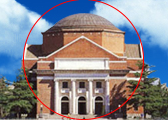
\includegraphics[width=.4\textwidth]{"../assets/1_circle.png"}
    }
    \quad
    \subfloat[绘制棋盘]{
        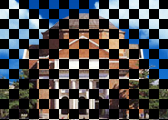
\includegraphics[width=.4\textwidth]{"../assets/1_grid.png"}
    }
    \caption{基础知识练习图像结果}
    \label{fig:exp1}
\end{figure}

\section{图像压缩编码}

\subsection{图像预处理}

对图像的预处理和二维DCT变换结合,记从原始图像中取得小块为P,DCT算子为D,最终系数为C,则过程为

\begin{align*}
    C & = D \cdot (P -
    \begin{bmatrix}
        128    & \cdots & 128    \\
        \vdots & \ddots & \vdots \\
        128    & \cdots & 128
    \end{bmatrix}
    ) \cdot D^T        \\
      & =DPD^T - D
    \begin{bmatrix}
        1      \\
        \vdots \\
        1
    \end{bmatrix}
    128
    \begin{bmatrix}
        1 & \cdots & 1
    \end{bmatrix}
    D^T
\end{align*}

将矩阵算子D与全1向量乘法展开,且注意到D中除了第一行外行和为0

\begin{align*}
    D_{N\times N}
    \begin{bmatrix}
        1      \\
        \vdots \\
        1
    \end{bmatrix}
     & =
    \sqrt{\frac{2}{N}}
    \begin{bmatrix}
        N\sqrt{\frac{1}{2}}                      \\
        \sum_{i=1}^N\cos{\frac{(2i - 1)\pi}{2N}} \\
        \vdots                                   \\
        \sum_{i=1}^N\cos{\frac{(N - 1)(2i - 1)\pi}{2N}}
    \end{bmatrix}
    =
    \begin{bmatrix}
        \sqrt{N} \\
        0        \\
        \vdots   \\
        0
    \end{bmatrix}
\end{align*}

代入C的计算式,得变换域的预处理方法

\begin{align*}
    C = DPD^T - 128
    \begin{bmatrix}
        N                 & 0_{1\times (N-1)}    \\
        0_{(N-1)\times 1} & 0_{(N-1)\times(N-1)}
    \end{bmatrix}
\end{align*}

化为Matlab代码,在图像中随机选取一块$8\times 8$的区域,分别进行空域和频域的处理,再使用2-范数衡量差异

\begin{minted}[bgcolor=bg]{matlab}
width = 8;
[h, w] = size(hall_gray);
D = dctmtx(width);

piece_x = floor(rand * (h - width) + 1);
piece_y = floor(rand * (w - width) + 1);
test_piece = double(hall_gray(piece_x(piece_x  + width - 1), ...
                              piece_y:(piece_y  + width - 1)));

% spatial domain
piece_sd = test_piece - 128;
dct_sd = D * piece_sd * D';

% frequency domain
dct_fd = D * test_piece * D';
dct_fd(1,1) = dct_fd(1,1) - 128 * width;

disp(norm(dct_sd - dct_fd));
\end{minted}

执行程序,得到的范数约为$1.5\times10^{-12}$,随机选取的小区域处理后的结果示例如图\ref{fig:exp2_1}

\begin{figure}[htb!]
    \centering
    \subfloat[空域处理]{
        
\includegraphics[width=.25\textwidth]{"../assets/2_1_sd.png"}
    }
    \qquad
    \subfloat[频域处理]{
        
\includegraphics[width=.25\textwidth]{"../assets/2_1_fd.png"}
    }
    \caption{图像DCT变换预处理结果}
    \label{fig:exp2_1}
\end{figure}

显然两种处理方式没有区别,都完成了预处理工作。考虑到代码的易读性,后面将更多采用空域处理的方式。

\subsection{二维DCT的实现}

分别实现\mintinline{matlab}{dct_mat}和\mintinline{matlab}{dct_2}两个函数,用于生成矩阵算子D和进行二维DCT。由于考虑的是对图片的正方形区域进行DCT,所以函数中进行判断确保输入为方阵。

\begin{minted}[bgcolor=bg]{matlab}
function D = dct_mat(N)
% DCT_MAT DCT N * N operator
% param N: width, height of the piece
% return D: N * N square matrix

t = 0 : N - 1;
D = cos(t' * (2 * t + 1) * pi / (2 * N));
D(1,:) = sqrt(0.5);
D = D * sqrt(2 / N);
end
\end{minted}

\begin{minted}[bgcolor=bg]{matlab}
function C = dct_2(P)
% DCT_2 2D discrete cosine transform
% param P: square matrix
% return C: transformed result

[w, h] = size(P);
assert(w==h, "P must be a square matrix");
P = double(P);
D = dct_mat(w);
C = D * P * D';
end
\end{minted}

再对\mintinline{matlab}{hall_gray}分别用Image Processing Toolbox中的\mintinline{matlab}{dct2}和前面实现的\mintinline{matlab}{dct_2}进行处理,使用2-范数衡量差异。

\begin{minted}[bgcolor=bg]{matlab}
mat_dct2 = @(block_struct) dct2(block_struct.data);
my_dct2 = @(block_struct) dct_2(block_struct.data);

mat_c = blockproc(img, [width width], mat_dct2, ...
                'PadPartialBlocks', true);
my_c = blockproc(img, [width width], my_dct2, ...
                'PadPartialBlocks', true);
\end{minted}

最终2-范数差异为$1.1133\times10^{11}$,可以认为功能一致。对\mintinline{matlab}{hall_gray}处理的结果见图\ref{fig:exp2_2}

\begin{figure}[htb!]
    \centering
    \subfloat[Matlab方法]{
        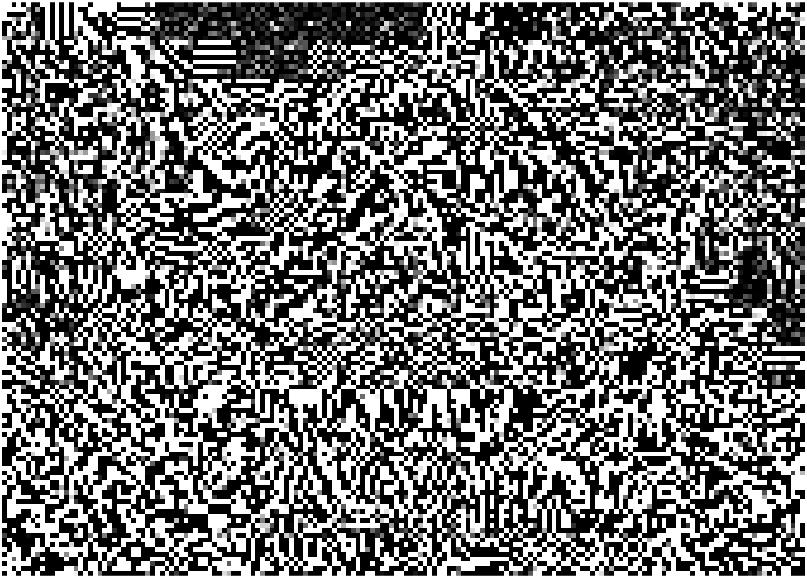
\includegraphics[width=.3\textwidth]{"../assets/2_2_matlab.png"}
    }
    \qquad
    \subfloat[自行实现方法]{
        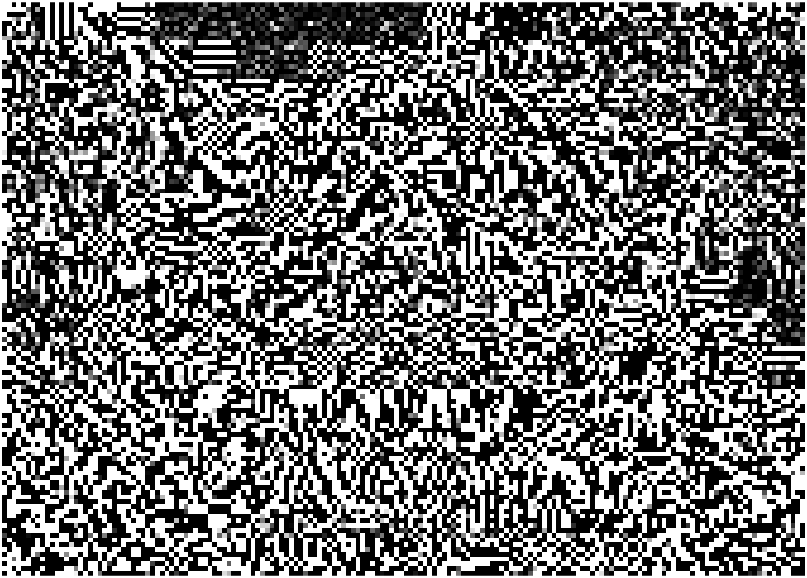
\includegraphics[width=.3\textwidth]{"../assets/2_2_my.png"}
    }
    \caption{二维DCT变换}
    \label{fig:exp2_2}
\end{figure}

\subsection{二维DCT系数矩阵性质1}\label{sec:2DDCT1}

将DCT处理后的系数矩阵左右四列分别置零,再经逆变换得到图像如图\ref{fig:exp2_3.1}

\begin{figure}[htb!]
    \centering
    \subfloat[左侧置零]{
        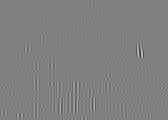
\includegraphics[width=.3\textwidth]{"../assets/2_3_inv_lz.png"}
        \label{fig:exp2_3_lz}
    }
    \qquad
    \subfloat[右侧置零]{
        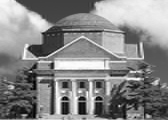
\includegraphics[width=.3\textwidth]{"../assets/2_3_inv_rz.png"}
        \label{fig:exp2_3_rz}
    }\\
    \subfloat[不置零]{
        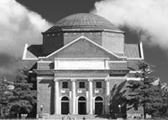
\includegraphics[width=.3\textwidth]{"../assets/2_3_inv.png"}
    }
    \qquad
    \subfloat[原始图像]{
        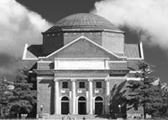
\includegraphics[width=.3\textwidth]{"../assets/2_3_origin.png"}
    }
    \caption{二维DCT变换系数矩阵变化的影响1}
    \label{fig:exp2_3.1}
\end{figure}

可以看到,左侧置零的结果图\ref{fig:exp2_3_lz}损失了大量人用来理解图像的原始信息,右侧置零的结果图\ref{fig:exp2_3_rz}则仍可清晰辨认。从DCT变换的原理来看,系数矩阵C的左上角为直流和低频分量,左下角为竖直高频和水平低频分量,右上角为竖直低频和水平高频分量,右下角为高频分量。当左侧置零时,水平方向的低频分量被消去,只剩高频分量,表现在测试图片上就是保留了明暗剧烈变化处的分界线;当右侧置零时,水平方向的高频分量被消去,只剩低频分量,表现在测试图片上就是明暗剧烈变化处模糊化。

提取横坐标57-64,纵坐标81-88的区域进行观察,如图\ref{fig:exp2_3.2}

\begin{figure}[htb!]
    \centering
    \subfloat[左侧置零]{
        
\includegraphics[width=.25\textwidth]{"../assets/2_3_inv_lz_p.png"}
        \label{fig:exp2_3_lz_p}
    }
    \quad
    \subfloat[右侧置零]{
        
\includegraphics[width=.25\textwidth]{"../assets/2_3_inv_rz_p.png"}
        \label{fig:exp2_3_rz_p}
    }
    \quad
    \subfloat[不置零]{
        
\includegraphics[width=.25\textwidth]{"../assets/2_3_inv_p.png"}
        \label{fig:exp2_3_inv_p}
    }
    \caption{二维DCT变换系数矩阵变化的影响2}
    \label{fig:exp2_3.2}
\end{figure}

相对于不置零的图\ref{fig:exp2_3_inv_p},右侧置零的图\ref{fig:exp2_3_rz_p}的水平变化看上去更加平滑,左侧置零的图\ref*{fig:exp2_3_lz_p}更加凸显了水平方向上的不同。这与前面的分析是一致的。

\subsection{二维DCT系数矩阵性质2}

对整张图的系数和对每一个$8\times8$的系数矩阵进行转置、旋转的操作,结果如图\ref*{fig:exp2_4}

\begin{figure}[htb!]
    \centering
    \subfloat[全图转置]{
        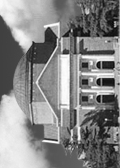
\includegraphics[width=.2\textwidth]{"../assets/2_4_inv_t.png"}
    }
    \quad
    \subfloat[全图旋转\ang{90}]{
        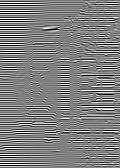
\includegraphics[width=.2\textwidth]{"../assets/2_4_inv_rot90.png"}
    }
    \quad
    \subfloat[全图旋转\ang{180}]{
        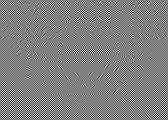
\includegraphics[width=.3\textwidth]{"../assets/2_4_inv_rot180.png"}
    }\\
    \subfloat[分块转置]{
        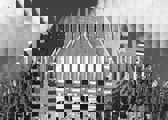
\includegraphics[width=.3\textwidth]{"../assets/2_4_inv_Ct.png"}
    }
    \quad
    \subfloat[分块旋转\ang{90}]{
        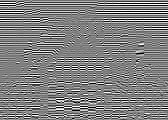
\includegraphics[width=.3\textwidth]{"../assets/2_4_inv_Crot90.png"}
    }
    \quad
    \subfloat[分块旋转\ang{180}]{
        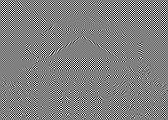
\includegraphics[width=.3\textwidth]{"../assets/2_4_inv_Crot180.png"}
    }
    \caption{二维DCT变换系数矩阵变化的影响3}
    \label{fig:exp2_4}
\end{figure}

除了全图的系数进行转置以外,都难以识别。考虑变换的过程,对系数矩阵C进行转置,只是将水平和竖直方向的系数做了交换,逆变换得到的结果也确实将水平和竖直方向的图案进行了“交换”,得到了将空域转置的效果。采用数学形式的描述即

\begin{align*}
    P   & = D^TCD     \\
    P^T & = (D^TCD)^T \\
        & =D^TC^TD
\end{align*}

而对每个$8\times8$的区域做转置,虽然同样符合此公式,但变换回空域后图案“不连续”,人难以识别该图片。

对于旋转\ang{90},由章节\ref*{sec:2DDCT1}中的分析,系数较大的直流与低频区域旋转至了竖直方向高频区域,故恢复的图像中由非常明显的横条纹,即竖直方向的剧烈变化。而旋转\ang{180}则将系数较大的直流与低频变换到了水平与竖直的共同高频区,造成了恢复后图像中大量的“棋盘状”黑白交替区域。

值得一提的是,全图系数旋转\ang{90}后,还能隐约看出与全图转置一致的结构信息。或许结构信息的分布经转置和旋转后差异较小,仍可以被识别。

\subsection{差分编码系统的频率响应}

该差分编码系统给出如下差分方程

\begin{align*}
    y(n) = x(n - 1) - x(n)
\end{align*}

对其进行Z变换,易得系统函数为

\begin{align*}
    H(z) = z^{-1} - 1
\end{align*}

故采用\mintinline{matlab}{freqz([-1, 1], 1)}函数绘制系统的频率响应如图

\begin{figure}[h]
    \centering
    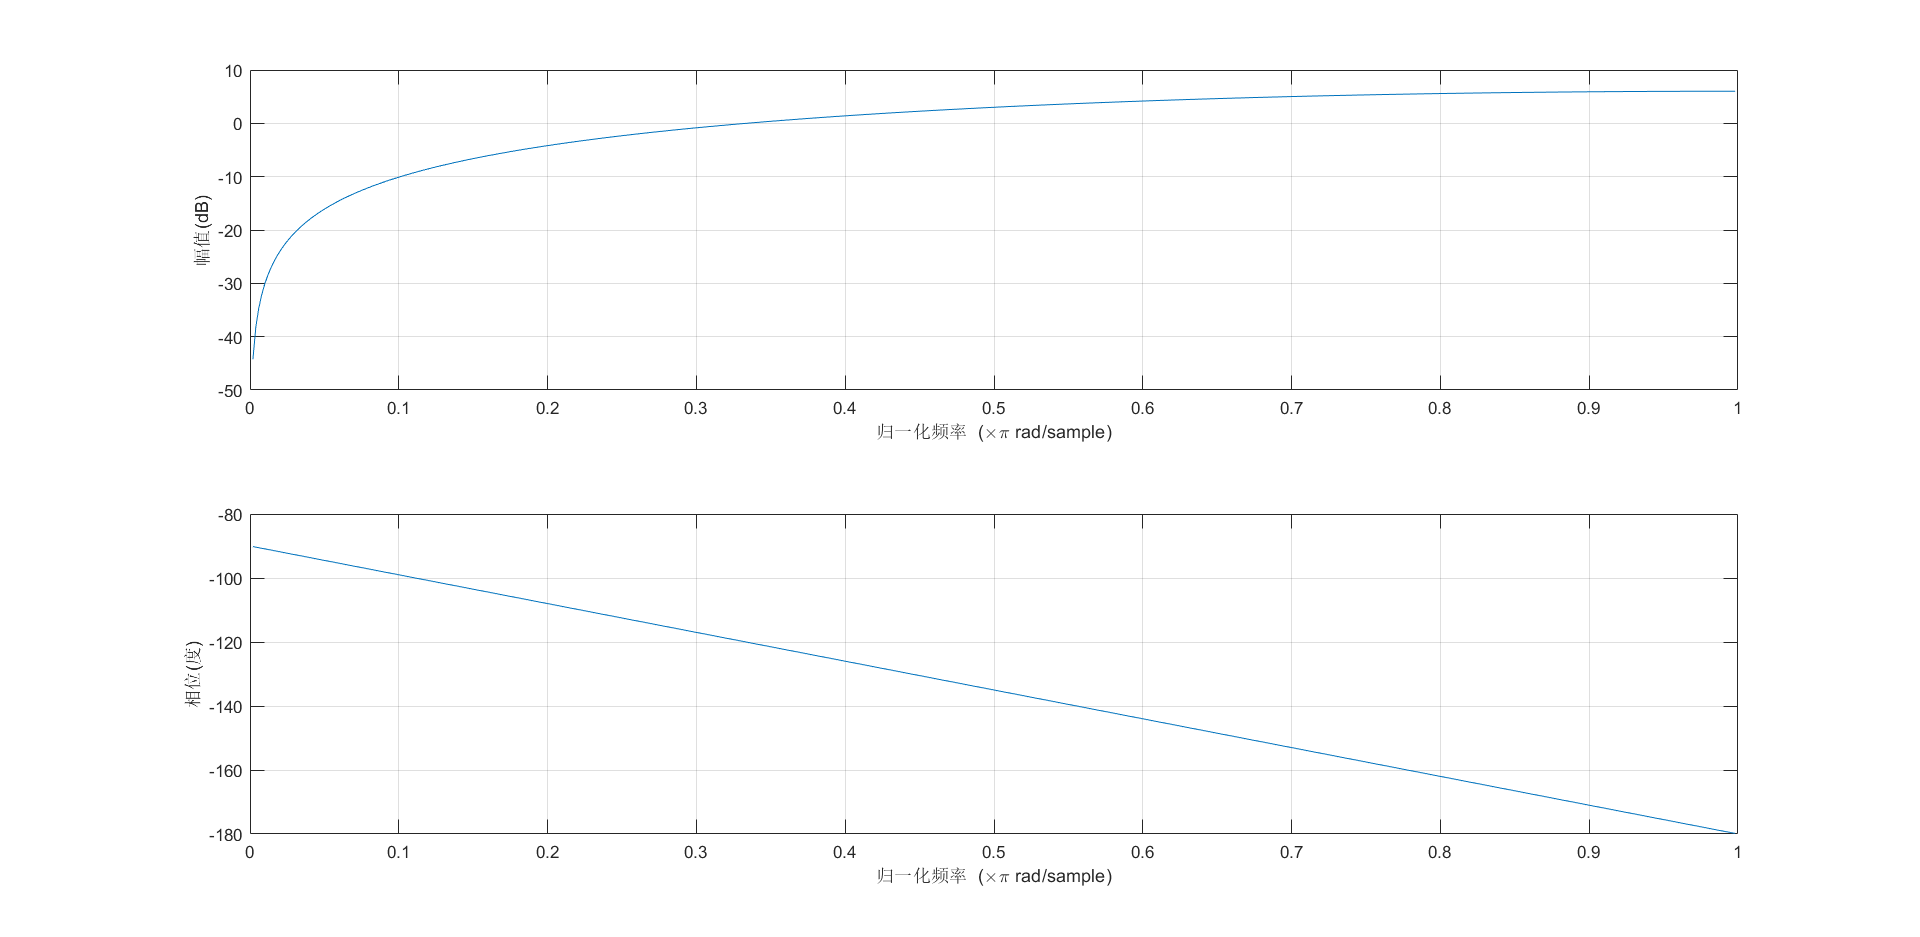
\includegraphics[width=.9\textwidth]{"../assets/2_5.png"}
    \caption{差分编码系统的频率响应}
    \label{fig:exp2_5}
\end{figure}

显然,这是一个高通系统,对DC系数进行差分编码便是为了略去过多的低频分量。

\subsection{DC预测的误差}

根据表格,易得二者间满足如下关系

\begin{align*}
    \text{category} = \lceil \log_2(|\text{预测误差}| + 1) \rceil
\end{align*}

对应到Matlab代码为

\begin{minted}[bgcolor=bg]{matlab}
category = ceil(log2(abs(x) + 1))
\end{minted}

需注意的是,上方代码给出的category从0开始,之后若需用作索引,应加1满足Matlab从1开始的规定。

\subsection{Zig-Zag扫描的实现}

考虑Zig-Zag扫描在压缩编码中使用的场景永远是$8\times8$的矩阵,可以简单的使用一个索引数组作为表,然后使用查表的方法进行扫描

\begin{align*}
    \text{index} =
    \begin{bmatrix}
        1 & 9 & 2 & \cdots & 56 & 64
    \end{bmatrix}
\end{align*}

考虑更一般的情形,可以对任意形状的矩阵使用循环,以$O(n^2)$的复杂度进行一轮Zig-Zag扫描。函数实现类似于

\begin{minted}[bgcolor=bg]{Matlab}
function output = zigzag(input)
    [r, c] = size(input);
    output = zeros(1, r * c);
    i = 1;
    j = 1;
    cnt = 1;
    
    while ((i <= r) && (j <= c))
        output(cnt) = input(i, j);
        cnt = cnt + 1;
        if (mod(i + j, 2))
            % odd => down
            if (i == r)
                j = j + 1;
            elseif (j == 1)
                i = i + 1;
            else
                i = i + 1;
                j = j - 1;
            end
        else
            % even => up
            if (j == c)
                i = i + 1;
            elseif (i == 1)
                j = j + 1;
            else
                i = i - 1;
                j = j + 1;
            end
        end
    end
end
\end{minted}

在Stack Overflow上面搜索后,找到了下方性能优异的实现方式\footnote{这两段代码将Stack Overflow上的问题\href{https://stackoverflow.com/questions/3024939/matrix-zigzag-reordering}{Matrix “Zigzag” Reordering}中Amro和Luis Mendo的答案改为函数。}

\begin{minted}[bgcolor=bg]{Matlab}
function output = zigzag_amro(input)
    ind = reshape(1:numel(input), size(input));
    ind = fliplr( spdiags( fliplr(ind) ) );
    ind(:,1:2:end) = flipud( ind(:,1:2:end) );
    ind(ind==0) = [];
    output = input(ind);
end
\end{minted}

\begin{minted}[bgcolor=bg]{Matlab}
function output = zigzag_luis(input)
    [r, c] = size(input);
    M = bsxfun(@plus, (1:r).', 0:c-1);
    M = M + bsxfun(@times, (1:r).'/(r+c), (-1).^M);
    [~, ind] = sort(M(:));
    output = input(ind).';
end
\end{minted}

其中Amro的实现方式利用\mintinline{matlab}{spdiags}函数将矩阵元素放在对角线上,从而将Zig-Zag扫描变为了竖直方向的扫描,再通过翻转特定的列实现了扫描方向的改变,最后删除0元素得到Zig-Zag矩阵作为索引。而Luis的实现方式巧妙的建立一个矩阵,其元素与其位置相关,大小按Zig-Zag扫描顺序排列,从而得到了一个索引矩阵。

这两种方法虽然巧妙、高效,但是在本次实验的流程中,并不比查表有优势,故此后将使用查表的方式实现Zig-Zag扫描。此外,在解码过程中需要将Zig-Zag扫描得到的序列还原,即还需要一个逆过程的表。逆过程的表可以使用如下方式创建

\begin{minted}[bgcolor=bg]{Matlab}
    zigzag_inv_ind = zeros(1, 64)
    zigzag_inv_ind(zigzag_ind) = 1:64
\end{minted}

即使用\mintinline{matlab}{zigzag_ind}作为索引矩阵,按照位置排列1-64。

\subsection{分块量化的实现}\label{sec:preprocess}

与前面一样,先构造一个处理函数,然后使用\mintinline{Matlab}{blockproc}实现分块处理,代码如下

\begin{minted}[bgcolor=bg]{Matlab}
img = double(hall_gray) - 128;
process = @(block_struct) dct_process(block_struct.ata, ...
                                      QTAB, zigzag_ind);

DCT = blockproc(img, [8 8], process, 'PadPartialBlocks', true);
DCT = reshape(DCT', size(DCT, 2), 64, []);
DCT = permute(DCT, [2, 1, 3]);
DCT = reshape(DCT, 64, []);

function output = dct_process(input, QTAB, zigzag_ind)
    C = dct_2(input);
    C_quant = round(C ./ QTAB);
    C_zigzag = C_quant(zigzag_ind);
    output = C_zigzag';
end
\end{minted}

这会得到一个64行的矩阵DCT,每列即每块经DCT处理和量化后的系数。

注意使用了\mintinline{matlab}{reshape}和\mintinline{matlab}{permute}将\mintinline{matlab}{blockproc}得到的矩阵改为需要的格式。这种方法参考了Stack Overflow的问题\href{https://stackoverflow.com/questions/24426686/matlab-reshape-horizontal-cat?r=SearchResults}{Matlab reshape horizontal cat}下Luis Mendo的回答。此方法巧妙地利用转置和\mintinline{matlab}{permute},利用Matlab矩阵列优先的特性,将\mintinline{matlab}{blockproc}得到的$64 m \times n$的矩阵先划分为m层$64\times n$的矩阵,再拼成一个$64\times mn$的矩阵,完成了行优先的变形。

\subsection{JPEG编码}

在章节\ref*{sec:preprocess}的基础上,加入编码的部分。因为使用Matlab中\mintinline{matlab}{dec2bin}等函数(封装为1补码并转换为向量),且编码长度不定,故编码采用一维向量不断扩展的方式,可能造成性能较低。

对于DC编码,有如下代码呈现的3个部分:

\begin{minted}[bgcolor=bg]{matlab}
DC_coef = coef(1, :);
DC_coef = [2 * DC_coef(1), DC_coef(1:end - 1)] - DC_coef;

dc_block_process = @(data) DC_process(data, DCTAB);
DC = arrayfun(dc_block_process, DC_coef, 'UniformOutput', false);
DC = cell2mat(DC);

function output = DC_process(input, DCTAB)
    category = ceil(log2(abs(input)+1)) + 1;
    huffman_code = DCTAB(category, ...
                         2:DCTAB(category, 1) + 1);
    dc_bin_mag = dec2bin_vec(input);
    output = [huffman_code, dc_bin_mag];
end
\end{minted}

第一部分将量化DC系数进行差分,第二部分使用\mintinline{matlab}{arrayfun}对所有系数进行编码再使用\mintinline{matlab}{cell2mat}连接,第三部分为编码的函数。

使用的\mintinline{matlab}{dec2bin_vec}为基于\mintinline{matlab}{dec2bin}和\mintinline{matlab}{bitcmp}实现的1补码进制转换。

\begin{minted}[bgcolor=bg]{matlab}
function bin_vec = dec2bin_vec(dec_int)
    if(dec_int > 0)
        bin_vec = split(dec2bin(dec_int), '');
        bin_vec = str2double(bin_vec(2:end - 1))';
    elseif(dec_int == 0)
        bin_vec = [];
    else
        bin_vec = dec2bin(bitcmp(abs(dec_int), 'uint16'));
        bin_vec = split(bin_vec(end ...
            - size(dec2bin(abs(dec_int)), ...
            2) + 1 : end), '');
        bin_vec = str2double(bin_vec(2:end - 1))';
    end
end
\end{minted}

AC编码做类似的处理,尚未找到方法替代循环实现其中的部分功能,且输出为不定长数组不能应用\mintinline{matlab}{blockproc},可能效率较低。行数较多,故略去,详见随报告附源代码。

\subsection{压缩比}

原图为$120\times168$的uint8矩阵,即有20160字节。经过JPEG压缩后为2031位DC码流与23073位AC码流,以二进制存储占据25104位,即3138字节,故压缩比约为6.42。考虑到还需添加图片宽高等信息,并存储码表,实际文件大小可能会稍大一些。

\subsection{JPEG解码}

解码主要分为DC解码、AC解码、重组为系数矩阵、逆DCT变换四个部分。

对于DC编码使用的Huffman码表,观察发现以下三类情况:

\begin{enumerate}
    \item 编码00,幅度0,序列00
    \item 编码三位,幅度序列长度为编码转十进制减1
    \item 编码多于3位,幅度序列长度为0索引加2
\end{enumerate}

故可以通过查找0出现的位置,判断编码类型,进而获取后面幅度的二进制表示。

\begin{minted}[bgcolor=bg]{matlab}
cnt = 1;
while(cnt <= blocks)
    if(all(DC(1:2) == [0 0]))
        % category 0 mag 0
        DC(1:2) = [];
    else
        zero_ind = find(DC==0, 1);
        if(zero_ind < 4)
            huffman_code = DC(1:3);
            DC(1:3) = [];
            zero_ind = bin2dec( ...
                            strjoin( ...
                                string(huffman_code), '')) - 1;
        else
            DC(1:zero_ind) = [];
            zero_ind = zero_ind + 2;
        end
        mag = bin_vec2dec(DC(1:zero_ind));
        DC_coeff(cnt) = mag;
        DC(1:zero_ind) = [];
    end
    cnt = cnt + 1;
end
\end{minted}

而对于AC编码,Huffman码表较为复杂,故采用\mintinline{matlab}{ismember}和\mintinline{matlab}{find}结合的方式,查找序列的前i位是否存在于表中。

\begin{minted}[bgcolor=bg]{matlab}
huffman(:) = 0;
for i = 1:16
    huffman(i) = AC(i);
    idx = find(ismember(ACTAB_code, huffman, 'rows'), 1);
...
\end{minted}

对解码后的系数矩阵进行\mintinline{matlab}{reshape}和\mintinline{matlab}{permute},然后再做逆变换,得到图像

\begin{minted}[bgcolor=bg]{matlab}
coef = [DC_coeff; AC_coeff];

inv_zigzag = @(block_struct) ...
    idct2(reshape(block_struct.data(zigzag_inv), [8 8]) .* QTAB);
coef = reshape( ...
       permute( ...
       reshape(coef, 64, blocksize(2), []), ...
           [2 1 3]), ...
               blocksize(2), [])';

inv_img = blockproc(coef, [64, 1], inv_zigzag);
img = uint8(inv_img(1:height, 1:width) + 128);
\end{minted}

对于解码得到的$64\times \text{blocks}$的系数矩阵,先使用\mintinline{matlab}{reshape},转换为$64\times \text{横向块数} \times \text{纵向块数}$的张量。再使用\mintinline{matlab}{permute}交换行列,以满足Matlab列优先的特性。最后使用\mintinline{matlab}{reshape}和转置变形为$64\text{纵向块数}\times\text{横向块数}$的矩阵。

然后利用之前存储的逆Zig-Zag扫描序列作为索引,再使用\mintinline{matlab}{reshape}将每个$64\times1$的系数向量恢复成$8\times 8$的方阵。再使用\mintinline{matlab}{blockproc}对所有块做反量化和逆DCT变换。最后裁切、加上128,再改为整型存储。

对\mintinline{matlab}{hall_gray}进行编解码的结果如图\ref{fig:exp2_11}。

\begin{figure}[h]
    \centering
    \subfloat[压缩]{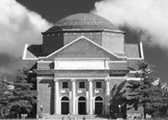
\includegraphics[width=.6\textwidth]{"../assets/2_11_decode.png"}}
    \quad
    \subfloat[原始]{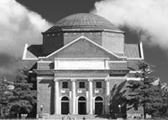
\includegraphics[width=.3\textwidth]{"../assets/2_11_origin.png"}}
    \caption{\mintinline{matlab}{hall_gray}编解码结果}
    \label{fig:exp2_11}
\end{figure}

经计算,PSNR为34.1878dB,失真应不算大。放大图片进行观察,经过编解码的图片中多出了一些噪声,也隐隐有了分块的边界。比较明显的如天空与云交界处,多出了许多噪点。云的颜色变化处有较为明显的分块特征。这或许正是JPEG压缩的特征:由分成若干个$8\times 8$的小块再编码的必然结果。

\subsection{量化步长的影响}

\begin{figure}[h]
    \centering
    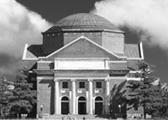
\includegraphics[width=.6\textwidth]{"../assets/2_12_decode.png"}
    \caption{\mintinline{matlab}{hall_gray}量化步长/2编解码}
    \label{fig:exp2_12}
\end{figure}

编码得到DC码流2408位,AC码流34156位,以二进制存储占36564位,即4570.5字节,压缩比约为4.41。相比前面的结果,压缩比上升,应是由于量化步长减半导致DC与AC系数较大,进而编码变长。

计算得到PSNR为37.1791dB,效果较前面的结果有所上升。实际观察噪声情况略有改善,但仍有分块边界。

\subsection{雪花图}

对雪花图进行编码,得到DC码流1403位,AC码流43539位,计算得压缩比约为3.65,PSNR为25.95dB。这表明雪花图接近随机数矩阵,有较多高频分量,量化造成的压缩失真较大。

考虑每个小块整个JPEG编解码的过程(使用$.*$和$./$表示逐元素乘除):

\begin{align*}
    \hat{P} = D^T (Q .* \text{round}(DPD^T ./ Q)) D
\end{align*}

失真由四舍五入导致,其幅度在0到量化步长之间。进一步考虑对每一块MSE的计算过程:

\begin{align*}
    MSE & = \frac{1}{64} \sum_i^8\sum_j^8 (P_{ij} - \hat{P_{ij}})^2                            \\
        & = \frac{1}{64} \sum (D^T (Q.*(DPD^T./Q - \text{round}(DPD^T ./ Q))) D).\hat{\quad} 2
\end{align*}

故由于四舍五入产生的误差将被Q放大到相应的量化步长,经过DCT逆变换后才得到MSE。中间的误差可以视为一系列在0到1之间均匀分布的随机数。

对于DCT逆变换,由于其为正交变换,且MSE的主干为Frobenius范数,由下式易知不会对结果产生影响:

\begin{align*}
    ||A||_F     & = \sqrt{\sum_{i=1}^m\sum_{j=1}^n a_{ij}} = \sqrt{\text{tr}(A^TA)}                                   \\
    ||D^TAD||_F & = \sqrt{\text{tr}((D^TAD)^T(D^TAD))}                                                                \\
                & = \sqrt{\text{tr}(D^TA^TDD^TAD)}                                   = \sqrt{\text{tr}((D^TA^T)(AD))} \\
                & = \sqrt{\text{tr}(ADD^TA^T)}                                       = \sqrt{\text{tr}(AA^T)}
\end{align*}

故MSE可以进一步转化为:

\begin{align*}
    MSE = \frac{1}{64}\sum(Q.*A).\hat{\quad} 2
\end{align*}

其中A为U(0,1)分布的随机数组成的矩阵。故可以计算其期望为:

\begin{align*}
    E(x) = \int_0^{0.5}x^2dx + \int_{0.5}^1(1-x)^2dx = \frac{1}{12}
\end{align*}

所以MSE的理论结果为$\sum(Q.\hat{\quad} 2)/(12\times 64) = 375.0365$,相应的PSNR为22.39dB。与对雪花图进行压缩的结果相近,这表明雪花图确实接近随机矩阵。

注意到对雪花图进行编码时,AC码流的长度较之前图像编码有了明显的上升,同时PSNR明显下降。推测是量化表中的系数经过设计,目的是对一般的图像中不太重要的高频信息进行滤波。而雪花图接近随机数注册的矩阵,量化表不适合对其进行处理,故最终压缩比相对较低。

\section{信息隐藏}

\subsection{空域隐藏}

使用\mintinline{matlab}{randi}生成一个随机01序列,并补0至长度与像素数一致。通过位移和加法,将像素最后一位替换为随机序列。经过JPEG编解码后与原有序列对比,记录正确率。代码如下

\begin{minted}[bgcolor=bg]{matlab}
parfor i = 1:100
    secret = randi([0, 1], 1, randi(max_length));
    len = length(secret);
    secret_pad = [secret, zeros(1, max_length - len)];
    
    encode = reshape(bitshift(bitshift(img, -1), 1), 1, []);
    encode = reshape(encode + secret_pad, size(img));
    [DC, AC, height, width] = ... 
        JPEG_encode(encode, QTAB, DCTAB, ACTAB, zigzag_ind);
    decode = ... 
        JPEG_decode(DC, AC, height, width, QTAB, ACTAB, zigzag_inv_ind);

    secret_decode = reshape(decode, 1, []);
    secret_decode = mod(secret_decode(1:len), 2);

    correct = correct + sum(secret_decode == secret) / len;
end
\end{minted}

最终得到正确率0.4996,可以认为是生成了一段新的随机序列替换原有序列,完全破坏了隐藏信息。所以空域隐藏法抗编解码能力弱,不适于当前的互联网环境。

\subsection{频域隐藏}

根据说明,实现了以下三种频域隐藏方法:

\begin{enumerate}[a)]
    \item \mintinline{matlab}{dct_embed_1}: 将二进制信息嵌入所有dct系数的最后一位
    \item \mintinline{matlab}{dct_embed_2}: 将二进制信息嵌入经Zig-Zag扫描后的dct系数从\mintinline{matlab}{bias}开始的\mintinline{matlab}{len}个系数的最后一位
    \item \mintinline{matlab}{dct_embed_3}: 将二进制信息变为1,-1序列,嵌入dct系数最后一个不为0数的后面一位
\end{enumerate}

三种方法的信息容量分别约为:像素数、像素数/64 - 像素数、像素数/64。

测试时对于\mintinline{matlab}{dct_embed_2}采取将信息嵌入2-9位系数,另外两种方法则使用基本满容量的信息进行嵌入。得到结果如图\ref{fig:exp3_2}和表\ref{tab:exp3_2}。

\begin{table}[h]
    \centering
    \caption{频域信息嵌入效果}
    \label{tab:exp3_2}
    \begin{tabular}{llll}
        \hline
                & 压缩比 & PSNR    & 正确率 \\ \hline
        embed 1 & 2.8561 & 18.7162 & 1      \\
        embed 2 & 6.2485 & 33.362  & 1      \\
        embed 3 & 6.1914 & 31.8924 & 1      \\ \hline
    \end{tabular}
\end{table}

\begin{figure}[h]
    \centering
    \subfloat[embed 1]{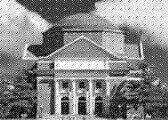
\includegraphics[width=.3\textwidth]{"../assets/3_2_embed_1.png"}}
    \quad
    \subfloat[embed 2]{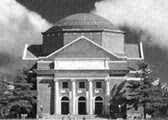
\includegraphics[width=.3\textwidth]{"../assets/3_2_embed_2.png"}}
    \quad
    \subfloat[embed 3]{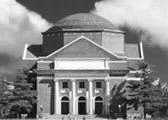
\includegraphics[width=.3\textwidth]{"../assets/3_2_embed_3.png"}}
    \caption{\mintinline{matlab}{hall_gray}频域信息嵌入结果}
    \label{fig:exp3_2}
\end{figure}

可以看到,方法2和3因为添加信息较少,且基本不会影响高频系数,故压缩比与未添加隐藏信息时相差无几。而方法一的质量和压缩比明显下降,并且人眼看来有明显的棋盘状图案,基本没有起到“隐藏”的意义。

由于是在频域进行嵌入,对于JPEG使用的DCT变换而言,这种嵌入可以保证信息无损。将信息尽可能嵌入中低频更有利于隐藏信息,即对于图像质量的影响尽可能低,对于压缩比的影响尽可能小。

\section{人脸检测}

\subsection{训练标准特征}

在生成颜色分布直方图时利用了所有像素,最后得到的频率分布与图像形状无关,故不需要调整图片形状,可以直接用于训练和检测。

使用如下函数得到一张图的颜色分布直方图,在计算所有训练数据的分布后求均值即可得到标准特征。

\begin{minted}[bgcolor=bg]{matlab}
function color_histogram = color_histogram(img, L)
%COLOR_HISTOGRAM generate color histogram of img
% param img: image matrix
% param L: color bit length <= 8
% return color_histogram: vector, histogram

[~, ~, c] = size(img);
assert(c == 3, 'img should have 3 channels, i.g. RGB');
bins = 0 : 2 ^ (3 * L);

img = floor(double(img) / 2 ^ (8 - L));
pixel = img(:, :, 1) * 2 ^ (2 * L) + ...
        img(:, :, 2) * 2 ^L + img(:, :, 3);
pixel = reshape(pixel, 1, []);

color_histogram = histcounts(pixel, bins) * 3 / numel(img);
end
\end{minted}

训练得到的标准特征如图\ref{fig:exp4_1}。可以看出,L的大小影响的是色彩空间聚集区域的数量。如L为3时,将RGB为0-31的数量聚集到[0, 0, 0],而L为4时该点聚集的是RGB为0-15的像素数量,L为5时聚集的是RGB为0-7的像素数量。L会影响到颜色空间密度分布聚集后表现出来的“分辨率”。

\begin{figure}[h]
    \centering
    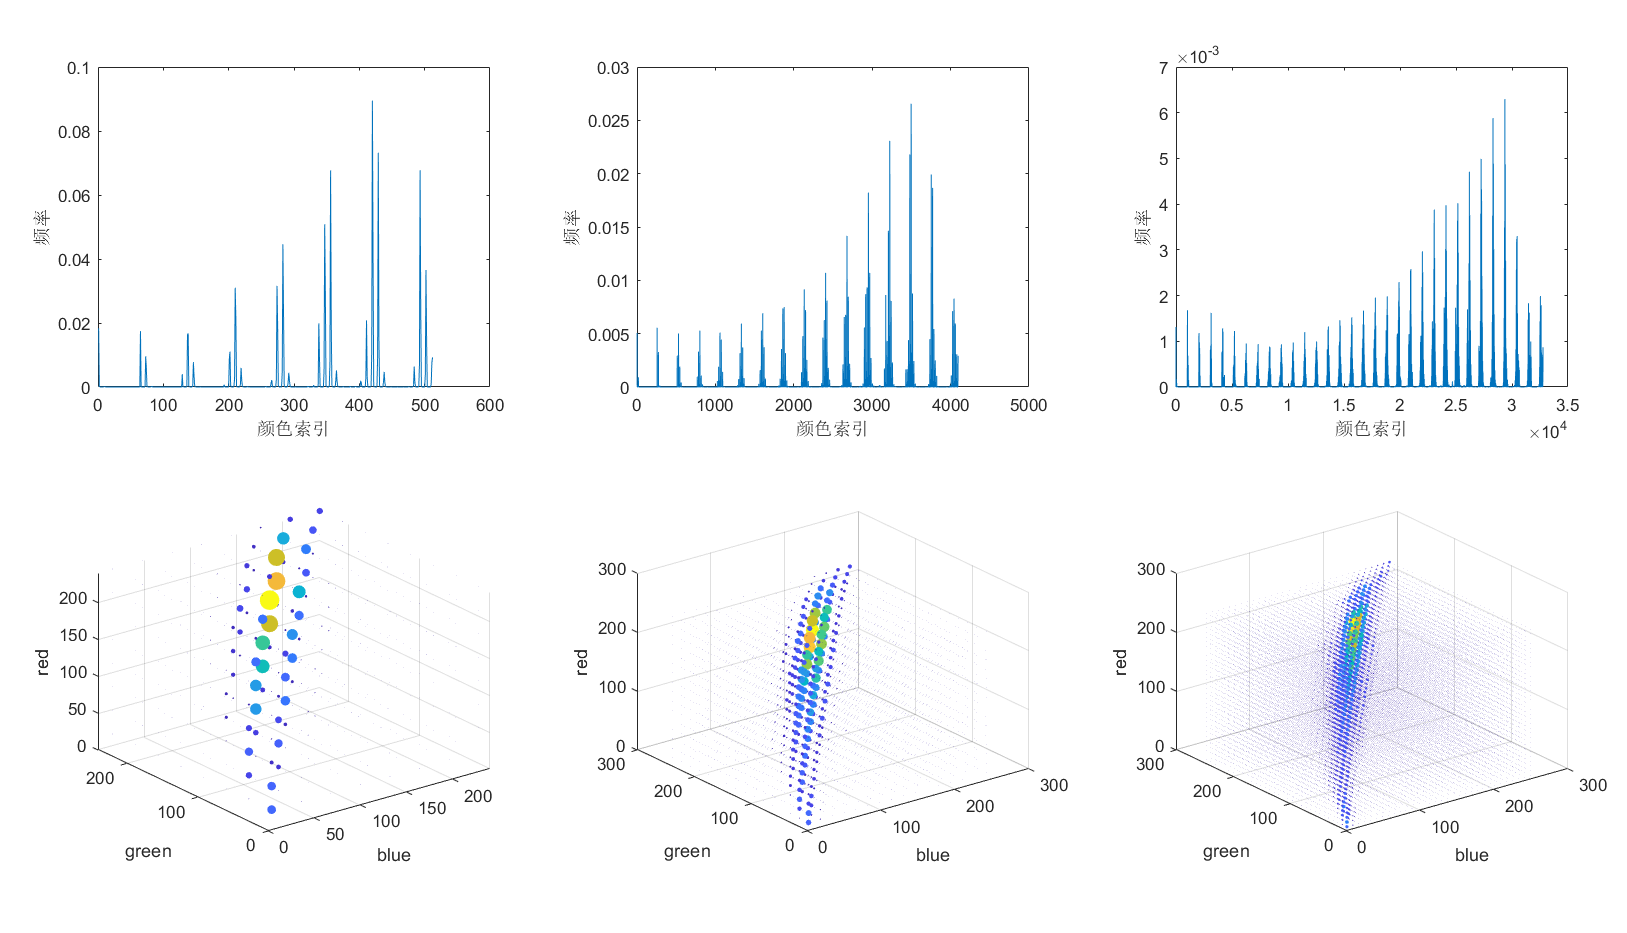
\includegraphics[width=.9\textwidth]{"../assets/4_1.png"}
    \caption{颜色分布直方图与颜色空间密度分布}
    \label{fig:exp4_1}
\end{figure}

\subsection{使用循环进行人脸检测}

下面尝试使用循环从图片中检测出人脸,为方便复用,构建一个函数:

\begin{minted}[bgcolor=bg]{matlab}
function candidates = ...
  detect_face(img, color_hist, L, blk_size, stride, threshold, k)
\end{minted}

此函数接受一个图片矩阵($H \times W \times C$),根据给定的颜色直方图标准color\_hist和参数L,对图片中的若干个区域(大小由blk\_size给定,数量由步长stride和图片尺寸给出)进行“特征距离”的计算,再返回小于阈值的前k个矩形位置经去除相交后的结果。流程大致如图\ref{fig:exp4_2_detect}所示,具体细节见随附代码。同时使用阈值和topK的目的是尽量限制去除相交区域时的候选矩形框数目,使其甚至可以少于k。实际使用时可以将阈值设为1,在全部的结果中选取k个,便可以规避因为阈值不合适得不到结果的问题。

\begin{figure}[h]
    \centering
    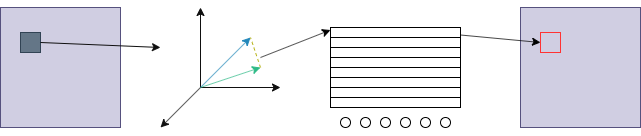
\includegraphics[width=.9\textwidth]{"../assets/detect.png"}
    \caption{人脸检测流程}
    \label{fig:exp4_2_detect}
\end{figure}

初步实验结果表明,由于L=5时直方图细节较多,距离普遍较大,需要适当调大阈值以得到相似的结果,否则可能会得不到任何结果。选用了一张阿森纳球队的合影,适当调整参数尽量检测出所有人,见图\ref{fig:exp4_2_result}。

\begin{figure}[ht!]
    \centering
    \subfloat[阿森纳合影原图]{
        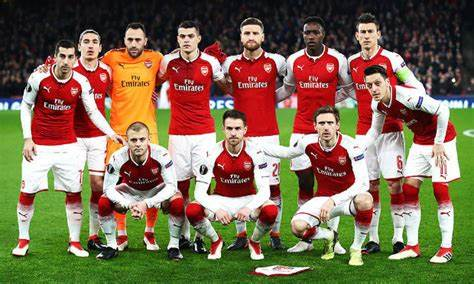
\includegraphics[width=.4\textwidth]{"../assets/Arsenal.jpg"}
    }
    \quad
    \subfloat[L=3 阈值0.4 k=50]{
        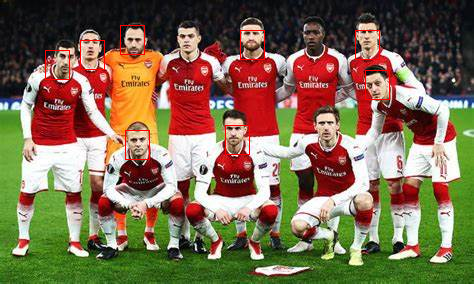
\includegraphics[width=.4\textwidth]{"../assets/4_2_L3.png"}
    }\\
    \subfloat[L=4 阈值0.4 k=100]{
        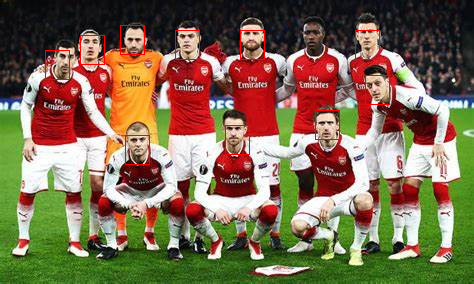
\includegraphics[width=.4\textwidth]{"../assets/4_2_L4.png"}
    }
    \quad
    \subfloat[L=5 阈值0.6 k=100]{
        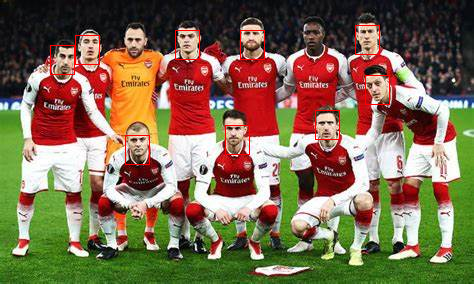
\includegraphics[width=.4\textwidth]{"../assets/4_2_L5.png"}
    }
    \caption{人脸检测结果\\$\text{blk\_size} = [30, 25];\text{stride} = [5, 5];$}
    \label{fig:exp4_2_result}
\end{figure}

可以看到,阈值和k足够大时,L并不太影响检测结果。由于函数中是先选出距离前k小的,再使用\mintinline{matlab}{rectint}和循环进行$O(n^2)$的相交区域去除,故L=3的结果可能由于此原因相比L=4多遗失了两名球员的结果。由于训练使用的样本肤色较浅,当前参数均没有识别出右上角肤色较深的球员,表明此方法有相当大的局限性。

\subsection{颜色分布直方图检测的稳定性}

在上一节中,L=3的效果已经不错,下面仍然使用L=3进行实验。使用以下函数对图像进行调整和检测:

\begin{minted}[bgcolor=bg]{matlab}
img_rotate = imrotate(img, 90);
img_resize = imresize(img, [size(img, 1), size(img, 2) * 2]);
img_adjust = imadjust(img, [.1 .15 0; .85 .9 1]);

candidates_rotate = ...
    detect_face(img_rotate, color_hist.vec_3, ...
        3, [25, 30], stride, 0.4, 100);
candidates_resize = ...
    detect_face(img_resize, color_hist.vec_3, ...
        3, [30, 50], stride, 0.4, 100);
candidates_adjust = ...
    detect_face(img_adjust, color_hist.vec_3, ...
        3, [30, 25], stride, 0.4, 100);
\end{minted}

\begin{figure}[ht!]
    \centering
    \subfloat[拉伸]{
        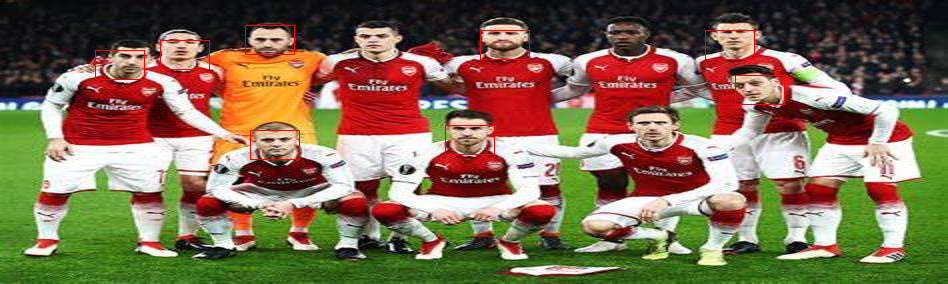
\includegraphics[width=.9\textwidth]{"../assets/4_3_resize.png"}
    }
    \\
    \subfloat[旋转]{
        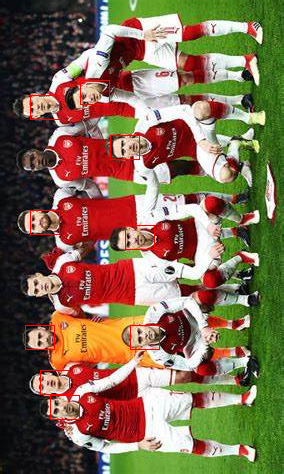
\includegraphics[width=.25\textwidth]{"../assets/4_3_rotate.png"}
    }
    \quad
    \subfloat[颜色调整]{
        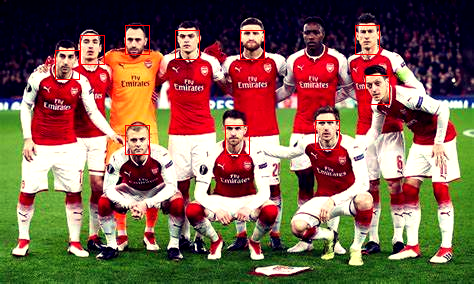
\includegraphics[width=.55\textwidth]{"../assets/4_3_adjust.png"}
    }
    \caption{人脸检测结果稳定性实验}
    \label{fig:exp4_3}
\end{figure}

从颜色分布直方图检测法的原理来看,旋转必然不会影响检测结果,而拉伸可能会由于插值方式的不同带来些微的影响,颜色调整则必然会带来影响。在图\ref{fig:exp4_3}中可以看到,旋转后的结果较上一节略好,这应是调大了k的结果。与之相比,拉伸少检测出一个人,调整颜色则多检测出一个人。这可能就是颜色的些微变化,让球员的脸部颜色直方图在所有候选中排位往前(或往后)移动,导致最后检测结果出现变化。

\subsection{人脸样本训练标准的选取}

从前面的实验结果来看,这种基于颜色分布直方图的方法虽然有受旋转、拉伸影响小的优点,但是非常受训练样本的影响,导致本实验中没有检测出非裔球员。虽然可能颜色分布与标准样本距离小于阈值,但仍会因为过于接近阈值,而在选取topK的步骤中被舍弃。如需进行更为准确的人脸检测,应当考虑针对不同人种训练不同的人脸标准,并在应用时将检测区域与所有样本进行比对,使得不同人种的脸部都能被识别出来。但随着标准的增多,误判的概率会有所上升,应考虑进一步限制阈值以保证准确性。

然而,由于颜色分布直方图的原理局限于颜色,不能捕获边缘特征。实际应用于人脸检测时应考虑引入边缘特征,与颜色分布一起计算一个“置信度”,再根据这个“置信度”决定是否是人脸。

\section{后记}



\end{document}